\documentclass[tikz,border=2pt]{standalone}
\usepackage{tikz}
\usepackage[european]{circuitikz}
\usetikzlibrary{arrows.meta,positioning,calc}
../cictikz/src/cictikz/data/tex/cictikz_lib.tex
\begin{document}
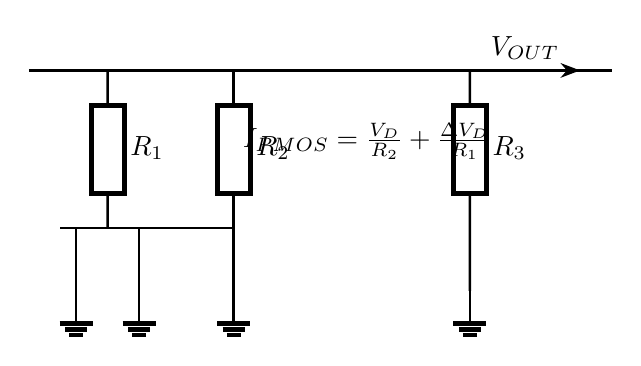
\begin{tikzpicture}[>=Stealth, line width=0.9pt]
  \draw (0,3.0) -- (7.4,3.0);
  \draw (1.0,3.0) to[resistor,l=$R_1$] (1.0,1.0);
  \draw (2.6,3.0) to[resistor,l=$R_2$] (2.6,1.0);
  \draw (0.4,1.0) -- (2.6,1.0);
  \draw (0.6,1.0) -- (0.6,0.2) node[ground] {};
  \draw (1.4,1.0) -- (1.4,0.2) node[ground] {};
  \draw (2.6,1.0) -- (2.6,0.2) node[ground] {};
  \draw (5.6,3.0) to[resistor,l=$R_3$] (5.6,1.0) -- (5.6,0.2) node[ground] {};
  \draw[->] (5.6,3.0) -- (7.0,3.0) node[midway,above] {$V_{OUT}$};
  \node at (4.3,2.1) {$I_{PMOS}=\frac{V_D}{R_2}+\frac{\Delta V_D}{R_1}$};
\end{tikzpicture}
\end{document}
